%%%%%%%%%%%%%%%%%%%%%%%%%%%%%%%%%%%%%%%%%%%%%%%%%%%%%%%%%%%%%%%%%%%%%%%%%%%%%%%%
%2345678901234567890123456789012345678901234567890123456789012345678901234567890
%        1         2         3         4         5         6         7         8

  % Comment this line out
                                                          % if you need a4paper
%\documentclass[a4paper, 10pt, conference]{ieeeconf}      % Use this line for a4
                                                          % paper

% \IEEEoverridecommandlockouts                              % This command is only
                                                          % needed if you want to
                                                          % use the \thanks command
% \overrideIEEEmargins
% See the \addtolength command later in the file to balance the column lengths
\documentclass{article}
\usepackage{amsmath}
% \usepackage{bm}	
\usepackage{graphicx}

\newtheorem{Assumption}{Assumption}
\newtheorem{Theorem}{Theorem}
\newtheorem{Condition}{Condition}
\newtheorem{Corollary}{Corollary}
\newtheorem{Definition}{Definition}
\newtheorem{Lemma}{Lemma}
%\newtheorem*{Proof*}{Proof}
%\newtheorem{Proof}{Proof}
\newtheorem{Proposition}{Proposition}
\newtheorem{Result}{Result}
\newtheorem{Remark}{Remark}

\usepackage{graphicx}
%\usepackage{booktabs}
%\usepackage{unicode-math}
%\setmathfont{XITS Math}
\usepackage{multirow}
\usepackage{mdwlist}
\newtheorem{theorem}{Theorem}
\newtheorem{definition}{Definition}
\newtheorem{lemma}{Lemma}
\newtheorem{proposition}{Proposition}
\newtheorem{corollary}{Corollary}
\newtheorem{assumption}{Assumption}
\newtheorem{remark}{Remark}
\usepackage{threeparttable}
%\usepackage{graphicx}
%\usepackage{enumitem}
\DeclareMathOperator*{\argmax}{arg\,max}
\usepackage{amsfonts}
\usepackage{amsmath}
\usepackage{hyperref}
%\usepackage[lined, boxed, commentsnumbered,ruled]{algorithm2e}
% \usepackage{bbm}
\usepackage{float}
\usepackage{caption}
% \usepackage{subcaption}
\usepackage{amssymb}
\usepackage{mathrsfs}
\usepackage{subfigure}
% \usepackage[utf8]{inputenc}
% \usepackage{booktabs,lipsum}
% \usepackage{hyperref}

\newcommand{\e}{\mathsf{end}}
\newcommand{\x}{\mathsf{x}}
\newcommand{\y}{\mathsf{y}}
\newcommand{\X}{\mathsf{X}}
\newcommand{\Y}{\mathsf{Y}}
\newcommand{\WE}{\mathsf{WE}}
\newcommand{\NS}{\mathsf{NS}}

\begin{document}
\subsection{Simulation}

To validate the analysis presented in the previous subsection, we applied various sequencing policies in Simulation of Urban Mobility.  %\cite{krajzewicz2010traffic}

In this section, we will validate the theoretical results by simulating the sequencing policies at the smart intersection. 

We use average time lost of vehicles in each simulation to evaluate the three sequencing policies. Time lost of vehicles can be divided into two parts: waiting time due to the approaching zone is full; time lost due to vehicles drive slower than the desired speed. We use SUMO to get average time lost of passing the intersection for different sequencing policies by performing the simulations. Fig x shows the simulation intersection in SUMO. The intersection is divided into two directions, west-east (WE) and south-north (SN), each direction has its vehicle flow. The generating time step $T_g$ is limited due to the depart delay. We let $T_g=2$ in our simulation. In each simulation, the generating possibility of each vehicle flow changes from 0 to 1 veh/T with step 0.1 veh/T, and the vehicle flows are generated randomly. 


\begin{figure}[H]
  \centering
  \includegraphics[width=0.3\textwidth]{intersection_SUMO.png}
  \caption{Simulation intersection in SUMO.}
  \label{fig:simulation_SUMO}
\end{figure}

% \begin{figure}[H]
%   \centering
%   \includegraphics[width=0.3\textwidth]{images/intersection_SUMO.png}
%   \caption{Simulation intersection in SUMO.}
%   \label{fig:simulation_SUMO}
% \end{figure}

\subsection{Overall Configurations}

We use a queue $Q$ to record the order of entry to the intersection for vehicles. For different sequencing policies, we will have different algorithm to decide the queue. The motions of vehicles will only be uniformly accelerated motions. The $n$th vehicle in the queue vehicle has a minimal time to enter the crossing zone, denotedd by $minT_n$, which can be divided into two parts, the acceleration time and the uniform time. The set time to enter the crossing zone of the $n$th vehicle in the queue is $T_n$. We calculate the time by $T_0=minT_0$, $T_n=T_{n-1}+\theta_ij$, when $n>0$. The $\theta_{ij}$ is the minimal headway, and the headway matrix in our simulation is:
\begin{align*}
  {\Theta} = 
\begin{bmatrix}
$$
0.4 & 2\\
2 & 0.4
$$
\end{bmatrix},
\end{align*}

For each vehicle, if $minT_n<T_n$, the vehicle will decelerate at a constant acceleration $a_D$; if $minT_n>T_n$, the vehicle will accelerate at a constant acceleration $a_A$. Nevertheless, the velocity of the vihicle is bounded by $[v_{min},\bar{v}]$, where $\bar{v}$ is the desired velocity. When the vehicle is at the maximum velocity, it won't have a positive acceleration. Similarly, when the vehicle is at the minimum velocity, it won't have a negative accerlation. As for the minimal velocity $v_{min}$, it is a function of the distance to the crossing zone for each vehicle, denoted as $v_{min}(x)$.  On the one hand, we don't want vehicles stop at the beginning of the approaching area since it will block the following vehicles. On the other hand, we need the minimal velocity of the vehicle to be 0 so that they can stop until their turn to enter the crossing zone. Therefore, an ideal function is that the value is not too small at the beginning and it will decrease to 0.  We use a segmentation function, where $x$ is the distance to the crossing zone and $L$ is the length of the approaching zone.

\begin{equation}
  v_{min}(x)=
  \begin{cases}
  \bar{v}*0.5&\mbox{x>10}\\
  \bar{v}*x/L&\mbox{x<10}
  \end{cases}
\end{equation}
For vihicles that have traversed the crossing zone, it will drives uniformly at $\bar{v}$ and be deleted from the queue $Q$.

\subsubsection{FIFO}
For the first-in-first-out(FIFO) policy, each vehicle will be appended at the end of the queue $Q$ as soon as it enter the approaching zone. 



\subsection{MS}

For the minimal switch-over(MS) policy, each vihilce will be append at the end of the queue $Q$ as soon as it enter the approaching zone. The set time to enter the crossing zone is immediately calculated by $T_n=minT_n$. Then we will reorder the queue: First, we find the vehicle $n$ with minimal set time $T_n$, which will be the next vehicle to enter the crossing zone. Then we will keep releasing vehicles that have same direction with vehicle $n$, until there is no vehilces on this direction or there are two vehicles, $m$ and $m+1$, that have a time gap that  $T_{m+1}-T_m>2*\theta_{ij}, i \neq j$ and the first vehicle $l$ on the other direction can squeeze into the gap, i.e. $minT_l<T_m+\theta_{ij}, i \neq j$. Then we will change the releasing direction of vehicles and repeat until all vihicles in the queue have been reordered. After we reorder the queue, we will also recalculate the new set time to enter the approaching zone for all vehicles in the queue. 

\subsection{LQF}
For the longer queue first(LQF) policy, 

\subsection{Results of Simulation}
The average total time of passing the intersection for different sequencing policies is shown in Fig. 2. 
\begin{figure*}
 \centering
 \subfigure[FIFO.]{
 \label{fig:subfig:a} 
 \includegraphics[width=1.9in]{1.png}}
 \hspace{0.02in}
 %
 \subfigure[MSO.]{
 \label{fig:subfig:c} 
 \includegraphics[width=1.9in]{2.png}}
 \hspace{0.02in}
 \caption{Heat map of average time lost for different sequencing policies;}
 \label{fig:SUMO_results} 
\end{figure*}


% \begin{figure*}
%  \centering
%  \subfigure[FIFO.]{
%  \label{fig:subfig:a} 
%  \includegraphics[width=1.9in]{images/FIFO.png}}
%  \hspace{0.02in}
%  %
%  \subfigure[MSO.]{
%  \label{fig:subfig:c} 
%  \includegraphics[width=1.9in]{images/MSO.png}}
%  \hspace{0.02in}
%  %
%  \subfigure[LQF.]{
%  \label{fig:subfig:b} 
%  \includegraphics[width=1.9in]{images/LQF.png}}
%  \hspace{0.02in}
%  %
%  \subfigure[]{
%  \label{fig:subfig:d} 
%  \includegraphics[width=0.26in]{images/colorscale.png}}
%  \caption{Heat map of average total passing time for different sequencing policies; the color bar in (d) (with unit sec) applies to all three maps.}
%  \label{fig:SUMO_results} 
% \end{figure*}

In all these cases, the average total passing time for each sequencing policy rises as the generating possibility rises. For small generating possibility, there is almost no difference. When generating possibility increases, the average total passing time for LQF increases rapidly and exceeds the passing time of the other two sequencing policies. Although the passing time for MSO is larger than FIFO at some points, the maximum average total passing time MSO reaches is smaller than that for FIFO, which indicates that MSO attains a larger capacity than FIFO. The simulation results are compliant with our theoretical analysis results in Section  that the system has the largest capacity under MSO policy, while under LQF policy, it has the smallest capacity. 
\end{document}